\section{解的表示}
\label{sec:ellip-representation}

能把解写成公式的情形不多，但它们最能说明解由什么决定。下面三种表示各借助一种结构：区间上可以直接积分，线性性允许把点源的响应叠加起来，自伴性允许沿特征函数分解。每个公式都有成立的前提，这些前提与公式一起说明。

\subsection{区间上的求解}
\label{sec:ellip-interval}

先看最简单的两点边值问题。给定$f\in C[0,1]$与边界值$g_0,g_1$，求$u\in C^2[0,1]$满足
\begin{equation}
 -u''=f\quad\text{于}\ (0,1),\qquad u(0)=g_0,\quad u(1)=g_1.
 \label{eq:ellip-interval-dirichlet}
\end{equation}

积分一次，$u'(0)$是一个待定常数，记为$C_1$：
\[
 u'(x)=C_1-\int_0^xf(s)\,\mathrm{d}s .
\]
再积分一次，把二重积分交换次序化成单重积分，$u(0)$是第二个常数：
\[
 u(x)=u(0)+C_1x-\int_0^x(x-s)f(s)\,\mathrm{d}s .
\]

代入左端条件，得到$u(0)=g_0$。代入右端条件，解出$C_1$：
\[
 C_1=g_1-g_0+\int_0^1(1-s)f(s)\,\mathrm{d}s .
\]

两个积分常数恰好被两个边界条件确定。代回去整理，解分成两部分：
\begin{equation}
 u(x)=\underbrace{g_0(1-x)+g_1x}_{\text{边界贡献}}
 +\underbrace{x\int_0^1(1-s)f(s)\,\mathrm{d}s-\int_0^x(x-s)f(s)\,\mathrm{d}s}_{\text{源项贡献}} .
 \label{eq:ellip-interval-solution}
\end{equation}

边界贡献是连接两个边界值的直线，满足$u''=0$。源项贡献在两端为零。这一分解来自线性：边界数据和源项可以分别处理，再把结果相加。

取$f=1$、$g_0=1$、$g_1=3$做一次手算。式~\eqref{eq:ellip-interval-solution}中的积分是
\[
 \int_0^1(1-s)\,\mathrm{d}s=\frac12,\qquad \int_0^x(x-s)\,\mathrm{d}s=\frac{x^2}2 .
\]
于是
\[
 u(x)=(1+2x)+\frac{x}{2}-\frac{x^2}{2}=1+2x+\frac{x(1-x)}{2},
\]
边界贡献是$1+2x$，源项贡献正是式~\eqref{eq:ellip-running-solution}。

唯一性也可以直接读出。若$u_1,u_2$都是解，差$w=u_1-u_2$满足$w''=0$和$w(0)=w(1)=0$。$w''=0$说明$w$是一次函数，两端为零的一次函数只能恒为零。

\paragraph{Neumann条件：相容性与不唯一}
把两端的条件都换成通量。按上一节的约定，外法向在$x=0$处指向左，在$x=1$处指向右，所以问题是
\begin{equation}
 -u''=f\quad\text{于}\ (0,1),\qquad -u'(0)=g_0,\quad u'(1)=g_1.
 \label{eq:ellip-interval-neumann}
\end{equation}
仍然积分一次，这次两端的条件都落在$u'$上，$u$本身一次也没有被约束。

对方程在$[0,1]$上积分，由牛顿--莱布尼茨公式，
\[
 \int_0^1f\,\mathrm{d}x=-u'(1)+u'(0)=-g_1-g_0 .
\]
也就是说，解若存在，数据必须满足
\begin{equation}
 \int_0^1f\,\mathrm{d}x+g_0+g_1=0.
 \label{eq:ellip-interval-compat}
\end{equation}

物理上这是总热量的收支：棒内总产热加上从两端流入的热量必须为零，否则温度不可能稳定。这样的条件称为\term{相容条件}（compatibility condition）。反过来，式~\eqref{eq:ellip-interval-compat}成立时，由$u'(x)=-g_0-\int_0^xf$定义的函数在$x=1$处恰好满足第二个条件，再积分一次就得到解，积分常数$c$可以任取。

取$f(x)=1-2x$，$g_0=g_1=0$。此时$\int_0^1f=0$，相容条件成立。积分得到
\[
 u'(x)=x^2-x,\qquad u(x)=\frac{x^3}{3}-\frac{x^2}{2}+c .
\]
图~\ref{fig:ellip-neumann-compat}(a)是不同$c$对应的解。整条曲线可以上下平移，因为方程和边界条件都只看导数。若要挑出一个代表，可以要求$\int_0^1u=0$，由$\int_0^1(x^3/3-x^2/2)\,\mathrm{d}x=-1/12$得到$c=1/12$。

\begin{BookInlineFigure}
  \centering
  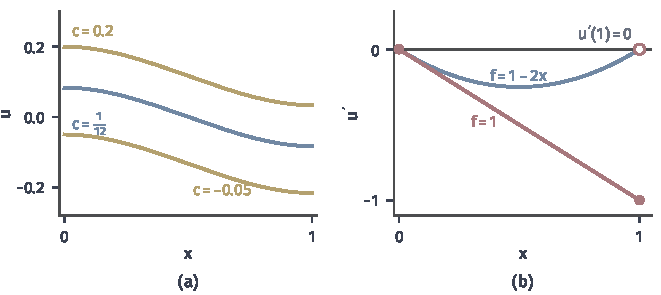
\includegraphics[width=112mm]{figures/06-differential-equations/02-partial-differential-equations/matplotlib/ellip-neumann-compat/figure.pdf}
  \caption{区间上的Neumann问题，$g_0=g_1=0$。(a)$f=1-2x$满足相容条件，解$x^3/3-x^2/2+c$可以任意平移；蓝线是零均值的代表，黄线是另外两个常数。(b)$u'$从$u'(0)=0$（红点）出发：$f=1-2x$时蓝线回到$u'(1)=0$（空心点）；$f=1$时红线走到$-1$，右端条件无法满足。}
  \label{fig:ellip-neumann-compat}
\end{BookInlineFigure}

若取$f=1$，图~\ref{fig:ellip-neumann-compat}(b)显示了失败的方式。从$u'(0)=0$出发，$u'(x)=-x$到右端变成$-1$，而边界要求$0$。两端绝热，棒内持续发热，温度只会不断上升，稳态根本不存在。

对比两种边界条件：Dirichlet问题对任何$f$都唯一可解，Neumann问题只在数据满足一个线性约束时可解，可解时解有一维的自由度。这与线性方程组$\bm{K}\bm{c}=\bm{b}$在$\bm{K}$奇异时的情形相同，后面会把这个对应写清楚。

\subsection{Green函数}
\label{sec:ellip-green}

式~\eqref{eq:ellip-interval-solution}中源项的贡献是对$f$的积分，说明解线性地依赖于$f$。线性依赖应该能写成“每一处的源乘以一个响应，再叠加”。这个响应是什么？

\paragraph{矩阵的逆给出点源响应}
把函数看成长向量，问题就变成矩阵方程。将$[0,1]$等分为$n+1$段，步长$h=1/(n+1)$，内部格点$x_i=ih$。用二阶差商近似$-u''$，边界值为零，得到$\bm{K}\bm{u}=\bm{f}$，其中
\begin{equation}
 \bm{K}=\frac1{h^2}\begin{pmatrix}2&-1&&\\-1&2&\ddots&\\&\ddots&\ddots&-1\\&&-1&2\end{pmatrix}.
 \label{eq:ellip-discrete-laplacian}
\end{equation}

解是$\bm{u}=\bm{K}^{-1}\bm{f}$，写成分量为$u_i=\sum_j(\bm{K}^{-1})_{i,j}f_j$。$\bm{K}^{-1}$的第$j$列，就是只在第$j$个格点放单位源时的整个解。求逆等于把每个格点上的点源响应都算好。

取$n=3$，$h=1/4$，可以手算：
\[
 \bm{K}=16\begin{pmatrix}2&-1&0\\-1&2&-1\\0&-1&2\end{pmatrix},\qquad
 \bm{K}^{-1}=\frac1{64}\begin{pmatrix}3&2&1\\2&4&2\\1&2&3\end{pmatrix}.
\]
每一列先升后降，顶点在对角元处，折线形如帐篷。矩阵对称，说明$y$处放源在$x$处的响应，等于$x$处放源在$y$处的响应。

\paragraph{区间上的点源}
让格点加密，这些帐篷收敛到什么？连续地提问：在$y\in(0,1)$处放一个单位点源，解$G(\cdot,y)$应当满足什么？点源之外没有源，所以$G(\cdot,y)$在$(0,y)$和$(y,1)$上都满足$u''=0$，都是一次函数。加上两端为零，可设
\[
 G(x,y)=\begin{cases}\alpha x,&0\leq x\leq y,\\ \gamma(1-x),&y\leq x\leq1 .\end{cases}
\]

在$y$处需要两个条件。第一，温度连续，否则温度有跳变，热流无穷大，这就是$\alpha y=\gamma(1-y)$。第二，把$-u''=f$在包含$y$的小区间上积分，右端是单位源的总量$1$，左端是$u'$在左右两侧之差的相反数，所以$u'$在$y$处向下跳$1$，这就是$\alpha+\gamma=1$。

两个方程解出$\alpha=1-y$，$\gamma=y$。于是
\begin{equation}
 G(x,y)=\begin{cases}x(1-y),&0\leq x\leq y,\\ y(1-x),&y\leq x\leq1 .\end{cases}
 \label{eq:ellip-green-1d}
\end{equation}
它称为这个边值问题的\term{Green函数}（Green's function）。第~\ref{chap:linear-differential-systems}章也有一个积分核，把脉冲输入变成后续响应，它在脉冲发生之前为零，体现因果。这里的$G$在点源两侧都不为零，因为边界条件把信息从两个方向都传了过来。

有了点源响应，一般的源就是点源的叠加：
\begin{equation}
 u(x)=\int_0^1G(x,y)f(y)\,\mathrm{d}y .
 \label{eq:ellip-green-1d-rep}
\end{equation}
图~\ref{fig:ellip-inverse-tent}验证了矩阵与函数的对应，$\bm{K}^{-1}$除以$h$后，每列的元素恰好落在$G$上。图~\ref{fig:ellip-tents-superposition}展示叠加：几个点源的帐篷相加，点源越多越接近真解。

\begin{BookInlineFigure}
  \centering
  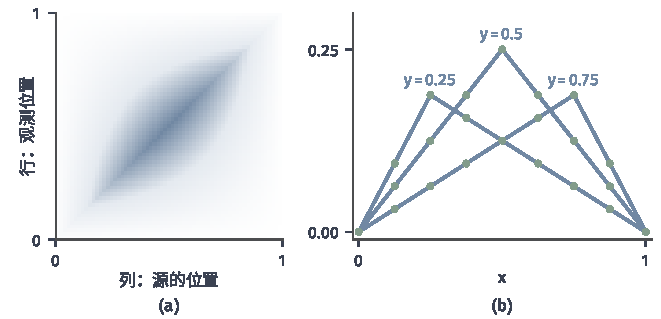
\includegraphics[width=112mm]{figures/06-differential-equations/02-partial-differential-equations/matplotlib/ellip-inverse-tent/figure.pdf}
  \caption{差分矩阵的逆是离散的Green函数。(a)$n=63$时$\bm{K}^{-1}/h$的取值，颜色越深值越大，沿对角线形成山脊。(b)$n=7$时第$2,4,6$列的元素（绿点）与式~\eqref{eq:ellip-green-1d}的$G(\cdot,y)$（蓝线），在格点上数值完全相同。}
  \label{fig:ellip-inverse-tent}
\end{BookInlineFigure}

现在验证式~\eqref{eq:ellip-green-1d-rep}。把积分在$y=x$处拆开，代入式~\eqref{eq:ellip-green-1d}：
\[
 u(x)=(1-x)\int_0^xyf(y)\,\mathrm{d}y+x\int_x^1(1-y)f(y)\,\mathrm{d}y .
\]

对$x$求导，积分限上出现的两项是$(1-x)xf(x)$和$-x(1-x)f(x)$，互相抵消，只剩
\[
 u'(x)=-\int_0^xyf(y)\,\mathrm{d}y+\int_x^1(1-y)f(y)\,\mathrm{d}y .
\]

再求导，得到
\[
 u''(x)=-xf(x)-(1-x)f(x)=-f(x).
\]
又由公式直接读出$u(0)=u(1)=0$。取$f=1$，
\[
 u(x)=(1-x)\frac{x^2}{2}+x\frac{(1-x)^2}{2}=\frac{x(1-x)}{2},
\]
这正是式~\eqref{eq:ellip-running-solution}。

\begin{BookInlineFigure}
  \centering
  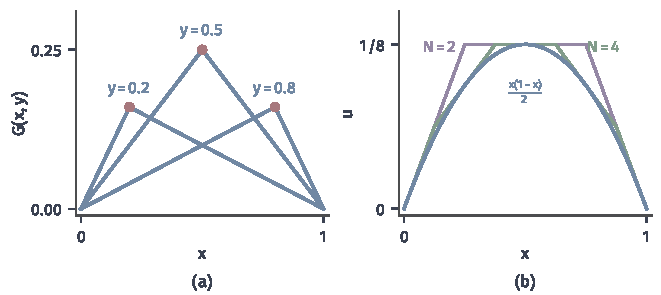
\includegraphics[width=112mm]{figures/06-differential-equations/02-partial-differential-equations/matplotlib/ellip-tents-superposition/figure.pdf}
  \caption{点源响应的叠加。(a)三个位置$y$处的单位点源产生的帐篷$G(\cdot,y)$，红点是顶点$(y,y(1-y))$。(b)均匀源$f=1$的离散近似：在$N$个等分小段的中点放权重$1/N$的点源，紫线$N=2$，绿线$N=4$，$N$增大时趋于蓝线$x(1-x)/2$。}
  \label{fig:ellip-tents-superposition}
\end{BookInlineFigure}

\paragraph{全空间的基本解}
多维情形不能分段积分，但点源响应的想法仍然有效。先在没有边界的全空间里问：单位点源在原点产生的平衡温度是什么？

对称性告诉我们解只依赖于到原点的距离$r=\lVert\bm{x}\rVert_2$，记为$\varphi(r)$。把所有热量想成从原点向外流：稳态下，单位热源产生的热量必须全部穿过每一个以原点为心的球面。半径$r$的球面面积是$d\omega_dr^{d-1}$，其中$\omega_d$是单位球的体积。所以径向热流密度为
\[
 -\varphi'(r)=\frac1{d\omega_dr^{d-1}} .
\]

积分一次，常数取最简单的值，就得到\termalias{基本解-偏微分方程}{基本解}（fundamental solution）
\begin{equation}
 \Phi(\bm{x})=\begin{cases}
 -\dfrac{\lVert\bm{x}\rVert_2}{2},&d=1,\\
 -\dfrac1{2\pi}\log\lVert\bm{x}\rVert_2,&d=2,\\
 \dfrac1{d(d-2)\omega_d}\,\lVert\bm{x}\rVert_2^{2-d},&d\geq3 .
 \end{cases}
 \label{eq:ellip-fundamental}
\end{equation}
$d=3$时$\omega_3=4\pi/3$，$\Phi=1/(4\pi\lVert\bm{x}\rVert_2)$。直接计算可知$\Delta\Phi=0$在原点之外成立：径向函数的Laplace是$r^{1-d}(r^{d-1}\varphi')'$，而$r^{d-1}\varphi'$是常数。

图~\ref{fig:ellip-fundamental-radial}比较了三个维数。维数越高，球面面积随半径增长越快，同样的热量摊得越薄，所以(b)中的流密度衰减得越快。$d=1$时热流不衰减，$\Phi$一直线性下降；$d\geq3$时$\Phi$在无穷远趋于零；$d=2$介于两者之间，$\Phi$对数发散。

\begin{BookInlineFigure}
  \centering
  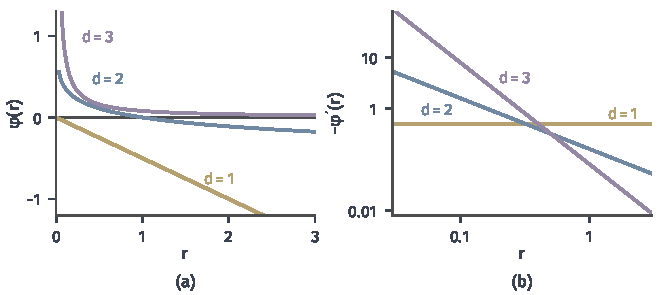
\includegraphics[width=112mm]{figures/06-differential-equations/02-partial-differential-equations/matplotlib/ellip-fundamental-radial/figure.pdf}
  \caption{基本解的径向形状。(a)$\varphi(r)$：$d=1$（黄）是直线，$d=2$（蓝）是对数，$d=3$（紫）是$1/(4\pi r)$，$d\geq2$时在原点发散。(b)流密度$-\varphi'(r)$的双对数图，斜率分别为$0,-1,-2$，体现单位热量摊在面积$d\omega_dr^{d-1}$上。}
  \label{fig:ellip-fundamental-radial}
\end{BookInlineFigure}

基本解只回答了全空间的问题。对紧支撑的$C^2$函数$f$，卷积
\[
 v(\bm{x})=\int_{\mathbb{R}^{d}}\Phi(\bm{x}-\bm{y})f(\bm{y})\,\mathrm{d}\bm{y}
\]
满足$-\Delta v=f$，这在下面的表示定理之后就能验证。但$v$不满足任何给定的边界条件。在$(0,1)$上取$f=1$，
\[
 v(x)=-\int_0^1\frac{\lvert x-y\rvert}{2}\,\mathrm{d}y=-\frac{x^2+(1-x)^2}{4},
\]
边界值$v(0)=v(1)=-1/4$不是$0$。它比真解$x(1-x)/2$处处低$1/4$，必须修正。

\paragraph{表示公式}
要知道边界怎样影响解，用Green第二恒等式。设$V$是有界区域，$\partial V$足够光滑，$u,w\in C^2(\overline V)$。向量场$u\nabla w-w\nabla u$的散度是
\[
 \nabla\cdot(u\nabla w-w\nabla u)=u\Delta w-w\Delta u .
\]
对它用散度定理，得到
\begin{equation}
 \int_V(u\Delta w-w\Delta u)\,\mathrm{d}\bm{x}=\int_{\partial V}(u\,\partial_{\bm{n}}w-w\,\partial_{\bm{n}}u)\,\mathrm{d}S,
 \label{eq:ellip-green-second}
\end{equation}
其中$\partial_{\bm{n}}w=\bm{n}\cdot\nabla w$是外法向导数。

我们想取$w=\Phi(\bm{x}-\cdot)$，但它在$\bm{x}$处奇异。办法是挖掉以$\bm{x}$为中心的小球，见图~\ref{fig:ellip-excised-ball}，在剩下的区域用恒等式，再让球缩小。

\begin{BookInlineFigure}
  \centering
  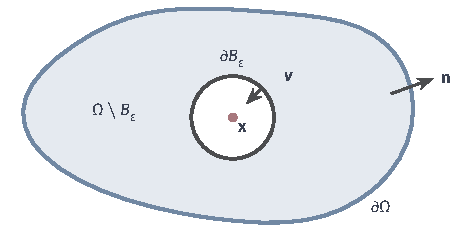
\includegraphics[width=78mm]{figures/06-differential-equations/02-partial-differential-equations/tikz/ellip-excised-ball/figure.pdf}
  \caption{挖去小球后的区域$\Omega\setminus B_\varepsilon$。外边界上的法向$\bm{n}$指向区域外，小球面上区域的外法向$\bm{\nu}$指向球心$\bm{x}$。}
  \label{fig:ellip-excised-ball}
\end{BookInlineFigure}

\begin{theorem}[Green表示公式]
\label{thm:ellip-representation}
设$d\geq2$，$\Omega\subset\mathbb{R}^{d}$是边界光滑的有界区域，$u\in C^2(\overline\Omega)$。则对每个$\bm{x}\in\Omega$，
\begin{equation}
 \begin{aligned}
 u(\bm{x})={}&\int_\Omega\Phi(\bm{x}-\bm{y})\bigl(-\Delta u(\bm{y})\bigr)\,\mathrm{d}\bm{y}\\
 &+\int_{\partial\Omega}\Bigl(\Phi(\bm{x}-\bm{y})\,\partial_{\bm{n}}u(\bm{y})-u(\bm{y})\,\partial_{\bm{n}}\Phi(\bm{x}-\bm{y})\Bigr)\,\mathrm{d}S(\bm{y}),
 \end{aligned}
 \label{eq:ellip-representation}
\end{equation}
其中法向导数对变量$\bm{y}$求。
\end{theorem}

\begin{proof}
固定$\bm{x}$，记$w(\bm{y})=\Phi(\bm{x}-\bm{y})$，取$\varepsilon$足够小使$\overline{B_\varepsilon(\bm{x})}\subset\Omega$，令$V=\Omega\setminus\overline{B_\varepsilon(\bm{x})}$。在$V$上$\Delta w=0$，式~\eqref{eq:ellip-green-second}化为
\[
 -\int_Vw\Delta u\,\mathrm{d}\bm{y}=\int_{\partial\Omega}(u\,\partial_{\bm{n}}w-w\,\partial_{\bm{n}}u)\,\mathrm{d}S+\int_{\partial B_\varepsilon}(u\,\partial_{\bm{\nu}}w-w\,\partial_{\bm{\nu}}u)\,\mathrm{d}S .
\]

在小球面上，$\bm{\nu}$指向球心，$w$的值是$\varphi(\varepsilon)$，方向导数是
\[
 \partial_{\bm{\nu}}w=-\varphi'(\varepsilon)=\frac1{d\omega_d\varepsilon^{d-1}},
\]
它正好是球面面积的倒数。于是第一项是$u$在球面上的平均值：
\[
 \int_{\partial B_\varepsilon}u\,\partial_{\bm{\nu}}w\,\mathrm{d}S=\frac1{\lvert\partial B_\varepsilon\rvert}\int_{\partial B_\varepsilon}u\,\mathrm{d}S\ \longrightarrow\ u(\bm{x}),\qquad\varepsilon\to0,
\]
极限成立是因为$u$连续。

第二项的绝对值不超过$\lvert\varphi(\varepsilon)\rvert\cdot d\omega_d\varepsilon^{d-1}\cdot\max\lVert\nabla u\rVert_2$。$d=2$时这是$\varepsilon\lvert\log\varepsilon\rvert$的倍数，$d\geq3$时是$\varepsilon$的倍数，都趋于零。

最后，$\Phi(\bm{x}-\cdot)$在$\bm{x}$附近可积，$\Delta u$有界，左端的积分当$\varepsilon\to0$时收敛到$\int_\Omega w\Delta u$的相反数。三个极限合起来，移项即得式~\eqref{eq:ellip-representation}。
\end{proof}

现在可以补上卷积的验证。设$f\in C_c^2(\mathbb{R}^{d})$，把导数放到$f$上，有$\Delta v=\Phi*\Delta f$。把定理用于$u=f$、足够大的球$\Omega$，边界项为零，给出$f=\Phi*(-\Delta f)$，所以$-\Delta v=f$。

式~\eqref{eq:ellip-representation}还不能算是解的公式，因为右端同时用到了边界上的$u$和$\partial_{\bm{n}}u$。对Dirichlet问题，$\partial_{\bm{n}}u$恰恰是未知的。要把它消掉。

\paragraph{区域的Green函数}
办法是给基本解加一个调和的修正，使修正后的函数在边界上为零，这样含$\partial_{\bm{n}}u$的项就消失了。

\begin{definition}[区域的Green函数]
\label{def:ellip-green-domain}
设$\Omega$是有界区域。若对每个$\bm{x}\in\Omega$，存在$h^{\bm{x}}\in C^2(\overline\Omega)$满足$\Delta h^{\bm{x}}=0$，且在$\partial\Omega$上$h^{\bm{x}}(\bm{y})=\Phi(\bm{x}-\bm{y})$，则称
\begin{equation}
 G(\bm{x},\bm{y})=\Phi(\bm{x}-\bm{y})-h^{\bm{x}}(\bm{y})
 \label{eq:ellip-green-domain}
\end{equation}
为$\Omega$上Dirichlet问题的Green函数。
\end{definition}

$\Phi$负责在点源处产生正确的奇性，$h^{\bm{x}}$负责抵消边界值。图~\ref{fig:ellip-green-corrector}在一维展示了这个构造：黄色的基本解在两端不为零，紫色的修正是过这两个端点值的直线，两者相减就是蓝色的帐篷。$\Phi$在全空间只有一个，而$G$随着区域变化，换一个区域就要重新解一次修正问题。

\begin{BookInlineFigure}
  \centering
  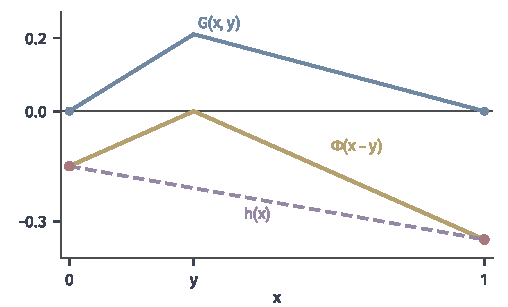
\includegraphics[width=86mm]{figures/06-differential-equations/02-partial-differential-equations/matplotlib/ellip-green-corrector/figure.pdf}
  \caption{一维Green函数的构造，$y=0.3$。黄线是基本解$\Phi(x-y)=-\lvert x-y\rvert/2$，红点是它的两个端点值。紫色虚线$h$是以这两个值为端点的直线，$h''=0$。蓝线$G=\Phi-h$在两端为零，就是式~\eqref{eq:ellip-green-1d}。}
  \label{fig:ellip-green-corrector}
\end{BookInlineFigure}

用$u$和$h^{\bm{x}}$再做一次式~\eqref{eq:ellip-green-second}，由$\Delta h^{\bm{x}}=0$得到
\[
 \int_\Omega h^{\bm{x}}\bigl(-\Delta u\bigr)\,\mathrm{d}\bm{y}=\int_{\partial\Omega}\bigl(u\,\partial_{\bm{n}}h^{\bm{x}}-h^{\bm{x}}\,\partial_{\bm{n}}u\bigr)\,\mathrm{d}S .
\]

用式~\eqref{eq:ellip-representation}减去这个等式。在边界上$\Phi=h^{\bm{x}}$，含$\partial_{\bm{n}}u$的两项抵消，得到
\begin{equation}
 u(\bm{x})=\int_\Omega G(\bm{x},\bm{y})\bigl(-\Delta u(\bm{y})\bigr)\,\mathrm{d}\bm{y}-\int_{\partial\Omega}u(\bm{y})\,\partial_{\bm{n}}G(\bm{x},\bm{y})\,\mathrm{d}S(\bm{y}) .
 \label{eq:ellip-green-rep}
\end{equation}

这个公式把解分成两份，第一份由源项产生，第二份由边界值产生。边界贡献不能省略，否则非零边值的信息就丢了。一维的验证很直接：端点$y=0$的外法向指向左，$\partial_{\bm{n}}G=-\partial_yG(x,0)=-(1-x)$，边界项给出$g_0(1-x)$；同样$y=1$处给出$g_1x$。两项合起来就是式~\eqref{eq:ellip-interval-solution}中的那条直线。

要小心公式的逻辑方向。式~\eqref{eq:ellip-green-rep}是说：\emph{如果}$C^2(\overline\Omega)$的解存在，\emph{并且}Green函数存在且足够光滑，解就必须是这个样子。它推出了唯一性，但没有证明存在性。

\paragraph{像源法}
几何特别简单时，修正项可以直接猜出来。考虑上半平面$\{x_2>0\}$，点源在$\bm{y}=(y_1,y_2)$。在边界另一侧的镜像点$\bm{y}^{*}=(y_1,-y_2)$放一个负的点源，由对称性，边界$x_2=0$上每一点到$\bm{y}$与到$\bm{y}^{*}$的距离相等，两个势在边界上抵消。这种做法称为\term{像源法}（method of images），二维的Green函数是
\begin{equation}
 G(\bm{x},\bm{y})=-\frac1{2\pi}\bigl(\log\lVert\bm{x}-\bm{y}\rVert_2-\log\lVert\bm{x}-\bm{y}^{*}\rVert_2\bigr).
 \label{eq:ellip-green-half-plane}
\end{equation}

半平面的外法向是$-\bm{e}_2$，把$-\partial_{\bm{n}}G=\partial_{y_2}G$在$y_2=0$处算出来：
\[
 P(\bm{x},y_1)=\frac{x_2}{\pi\bigl((x_1-y_1)^2+x_2^2\bigr)} .
\]
边界数据$g$产生的解是
\[
 u(\bm{x})=\int_{\mathbb{R}}P(\bm{x},y_1)\,g(y_1)\,\mathrm{d}y_1 ,
\]
$P$称为半平面的\term{Poisson核}（Poisson kernel）。半平面无界，这个公式对有界连续的$g$给出有界调和函数，要证明解确实取到边界值，需要对$P$的集中性质单独做极限估计，这里不细述。

图~\ref{fig:ellip-image-method}(b)说明Poisson核是一个加权平均：离边界越近，权重越集中在最近的边界点附近。这与解的边值恰好是$g$相吻合。离边界越远，权重摊得越开，解越光滑。

\begin{BookInlineFigure}
  \centering
  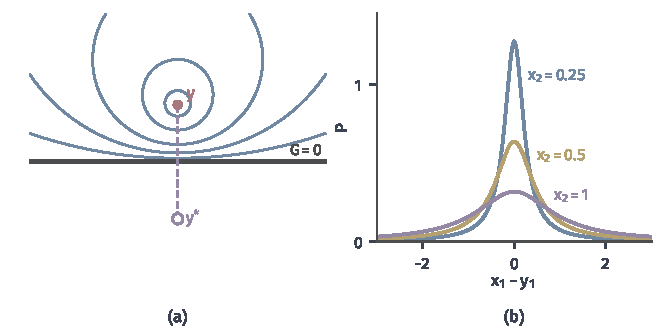
\includegraphics[width=112mm]{figures/06-differential-equations/02-partial-differential-equations/matplotlib/ellip-image-method/figure.pdf}
  \caption{上半平面的Green函数。(a)红点$\bm{y}=(0,1)$是点源，紫色空心点$\bm{y}^{*}=(0,-1)$是虚设的负像源，蓝线是$G$的等值线，粗线是边界，边界上$G=0$。(b)Poisson核$P$随$x_1-y_1$的变化，$x_2$越小峰越尖；每条曲线下的面积都是$1$。}
  \label{fig:ellip-image-method}
\end{BookInlineFigure}

\subsection{谱展开}
\label{sec:ellip-spectral}

Green函数把解写成“一处一处”的叠加。另一种思路是“一个模式一个模式”地叠加：找一组基，使微分算子在这组基下成为对角的，求解就成了逐个系数的除法。这正是对称矩阵的做法。

\paragraph{从矩阵的对角化到函数}
若$\bm{K}$对称正定，$\bm{K}=\bm{Q}\bm{\Lambda}\bm{Q}^\top$，那么$\bm{K}\bm{u}=\bm{f}$的解是把$\bm{f}$在特征向量上分解，每个分量除以对应的特征值，再合成。连续的对应物是
\begin{equation}
 -\Delta e_k=\lambda_ke_k\quad\text{于}\ \Omega,\qquad e_k=0\quad\text{于}\ \partial\Omega .
 \label{eq:ellip-eigenproblem}
\end{equation}

在区间$(0,1)$上，满足这个问题的函数和特征值是
\[
 e_k(x)=\sqrt2\sin(k\pi x),\qquad\lambda_k=k^2\pi^2,\qquad k\geq1 .
\]
这组函数是$L^2(0,1)$的标准正交基，它与Fourier级数的完备性同源，可参考\BookChapterRef{chap:fourier-transform}{卷四第14章“Fourier变换”}。把$f$与$u$按这组基展开，系数记为$f_k=\langle f,e_k\rangle$，$u_k=\langle u,e_k\rangle$。

用$e_k$乘方程$-u''=f$并积分，分部积分两次。$u$和$e_k$在端点都为零，边界项消失，得到
\[
 f_k=\int_0^1(-u'')e_k\,\mathrm{d}x=\int_0^1u(-e_k'')\,\mathrm{d}x=\lambda_ku_k .
\]
于是
\begin{equation}
 u=\sum_{k\geq1}\frac{f_k}{\lambda_k}\,e_k .
 \label{eq:ellip-spectral-solution}
\end{equation}

这个过程用到了边界条件的自伴结构：分部积分时$u$和$e_k$的边界项同时消失，$-\mathrm{d}^2/\mathrm{d}x^2$才能从$u$移到$e_k$上。对一般的有界区域，这样一组基是否存在，要等弱解理论建立之后才能回答。

\paragraph{一个完整的计算}
继续用$f=1$。系数是
\[
 f_k=\sqrt2\int_0^1\sin(k\pi x)\,\mathrm{d}x=\frac{\sqrt2\,(1-(-1)^k)}{k\pi} .
\]
偶数$k$的系数为零，奇数$k$的系数为$2\sqrt2/(k\pi)$。代入式~\eqref{eq:ellip-spectral-solution}，
\[
 u(x)=\sum_{k\ \text{奇}}\frac{4}{k^3\pi^3}\sin(k\pi x).
\]

在中点$x=1/2$处算几项部分和。$\sin(k\pi/2)$对$k=1,3,5$依次是$1,-1,1$，于是
\[
 \frac4{\pi^3}\approx0.12901,\qquad
 \frac4{\pi^3}\Bigl(1-\frac1{27}\Bigr)\approx0.12423,\qquad
 \frac4{\pi^3}\Bigl(1-\frac1{27}+\frac1{125}\Bigr)\approx0.12526 ,
\]
正在收敛到式~\eqref{eq:ellip-running-solution}给出的$1/8=0.125$。

图~\ref{fig:ellip-modes-coeffs}对比了$f$与$u$的系数。$f_k$按$1/k$衰减，所以部分和在间断处有明显的振荡，这是$f$在端点从$1$跳到边界值$0$的结果。$u_k=f_k/\lambda_k$按$1/k^3$衰减，只取第一项就已经和真解很接近。

除以$\lambda_k$压低高频，这就是椭圆问题的光滑作用。解比数据多出两阶导数的正则性，这在系数上表现为多出$k^{-2}$的衰减。

\begin{BookInlineFigure}
  \centering
  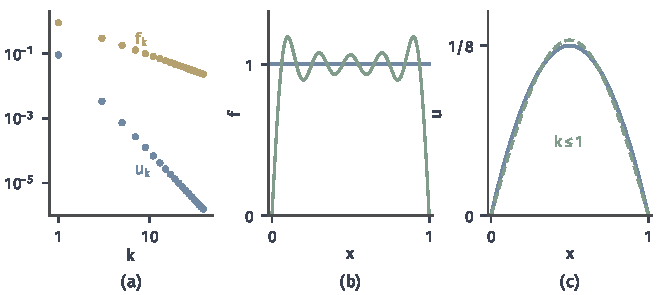
\includegraphics[width=112mm]{figures/06-differential-equations/02-partial-differential-equations/matplotlib/ellip-modes-coeffs/figure.pdf}
  \caption{$f=1$的正弦展开。(a)奇数$k$上$f_k$（黄）与$u_k=f_k/\lambda_k$（蓝）的双对数图，衰减率分别是$k^{-1}$与$k^{-3}$。(b)$f$的$k\leq9$部分和（绿）在$f$的目标值（蓝）附近振荡。(c)$u$的第一项（绿色虚线）已贴近真解（蓝）。}
  \label{fig:ellip-modes-coeffs}
\end{BookInlineFigure}

$f\in L^2(0,1)$时，式~\eqref{eq:ellip-spectral-solution}在$L^2$意义下收敛，它的导数级数也在$L^2$中收敛，这由下面两个有限的和保证：
\[
 \sum_k\frac{f_k^2}{\lambda_k^2}\leq\frac1{\lambda_1^2}\sum_kf_k^2<\infty,\qquad
 \sum_k\lambda_ku_k^2=\sum_k\frac{f_k^2}{\lambda_k}<\infty .
\]
逐点收敛和逐项求二阶导需要$f$有更多的光滑性，不能仅凭$f\in L^2$断言。

把$u_k=f_k/\lambda_k$的定义代回，再交换求和与积分，还能读出Green函数的谱表示：
\begin{equation}
 G(x,y)=\sum_{k\geq1}\frac{e_k(x)\,e_k(y)}{\lambda_k},
 \label{eq:ellip-green-spectral}
\end{equation}
这是矩阵等式$\bm{K}^{-1}=\sum_k\bm{q}_k\bm{q}_k^\top/\lambda_k$的函数版本。两种表示说的是同一个算子，一个按位置分解，一个按频率分解。

\paragraph{矩形区域}
积分区域是矩形时，变量分离给出二维的特征函数。在单位正方形上，
\[
 e_{m,n}(x_1,x_2)=2\sin(m\pi x_1)\sin(n\pi x_2),\qquad \lambda_{m,n}=\pi^2(m^2+n^2).
\]

若$f$恰好是单个模式，如$f=\sin(\pi x_1)\sin(\pi x_2)$，解就是$u=f/(2\pi^2)$，一次除法完成。取$f=1$，系数只在$m,n$都是奇数时非零，计算与一维相同，
\begin{equation}
 \begin{gathered}
 u(x_1,x_2)=\sum_{m,n\ \text{奇}}c_{m,n}\sin(m\pi x_1)\sin(n\pi x_2),\\
 c_{m,n}=\frac{16}{\pi^4mn(m^2+n^2)} .
 \end{gathered}
 \label{eq:ellip-square-series}
\end{equation}
图~\ref{fig:ellip-square-series}显示解的形状和中心点的收敛。第一项给出的中心值是$16/(2\pi^4)\approx0.0821$，加入更多项后趋于约$0.0737$。

\begin{BookInlineFigure}
  \centering
  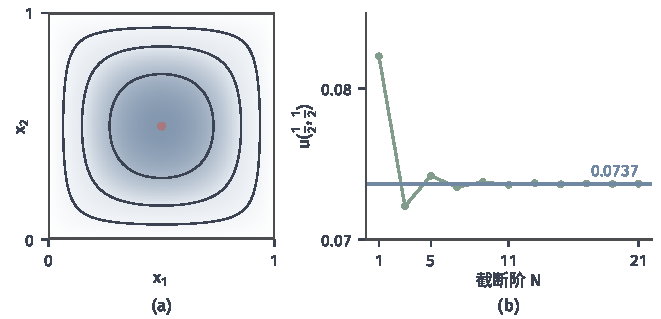
\includegraphics[width=112mm]{figures/06-differential-equations/02-partial-differential-equations/matplotlib/ellip-square-series/figure.pdf}
  \caption{单位正方形上$-\Delta u=1$、零Dirichlet边界的解。(a)$u$的取值，颜色越深值越大，等值线取$0.02,0.04,0.06$；角点附近的等值线被挤成圆角，红点是中心。(b)式~\eqref{eq:ellip-square-series}取$m,n\leq N$的中心值（绿）趋于蓝线。}
  \label{fig:ellip-square-series}
\end{BookInlineFigure}

\paragraph{零特征值}
把边界条件换成Neumann条件，特征问题的解变成$e_0=1$和$e_k=\sqrt2\cos(k\pi x)$，$\lambda_0=0$，$\lambda_k=k^2\pi^2$。式~\eqref{eq:ellip-spectral-solution}的第$k=0$项要除以$0$，不能直接用。

回到$\lambda_ku_k=f_k$这个关系，它对$k=0$说的是
\[
 0\cdot u_0=f_0=\int_0^1f\,\mathrm{d}x .
\]
这个等式有解当且仅当$f_0=0$，即相容条件~\eqref{eq:ellip-interval-compat}（$g_0=g_1=0$时）；一旦成立，$u_0$可以任取，这正是相差常数的不唯一。所以要先检查核空间上的分量，再对非零特征值做除法。

以$f=1-2x$为例，$f_0=0$，其余系数由分部积分算出，奇数$k$时$f_k=4\sqrt2/(k\pi)^2$，偶数$k$（$k\geq2$）时$f_k=0$。于是零均值的解是
\[
 u(x)=\sum_{k\ \text{奇}}\frac{8}{k^4\pi^4}\cos(k\pi x).
\]
在$x=0$处，第一项是$8/\pi^4\approx0.0821$，加上$k=3$的一项后约为$0.0831$，与前面的精确值$u(0)=1/12\approx0.0833$一致。
